\chapter[Proposta]{Proposta}

O principal objetivo deste trabalho é a construção de um framework modular para acesso a diferentes tipos de máquinário
utilizando um componente de baixo custo, no caso o ESP32, via comunicação \ac{MQTT}, para isso foram desenvolvidas algumas 
bibliotecas modulares que podem ser utilizadas para controlar três funções vitais do microcontrolador, de forma a 
tranformá-lo em um componente capaz de funcionar como um intermediário na comunicação do maquinário com a rede em nuvem; 
sendo, neste trabalho, a proposta dividir todo o código em três bibliotecas principais:

\section{ESP-Wifi}

Responsável por gerenciar o acesso dos ESP32 na rede Wifi, importante pois facilita o acesso a rede wifi utilizada 
gerenciando internamente o modelo de acesso que a depender do local e do tipo do experimento mudava de \ac{WPA2-PSK}
para \ac{WPA2-ENT}, vale ressaltar que entre os vários protocolos utilizados no \ac{WPA2-ENT} preferia-se sempre o uso do 
\ac{PEAP-MSCHAPv2}. A \autoref{fig:wifi} apresenta uma representação do sistema de heranças utilizado na biblioteca.

\begin{figure}[htb]
    \begin{center}
	    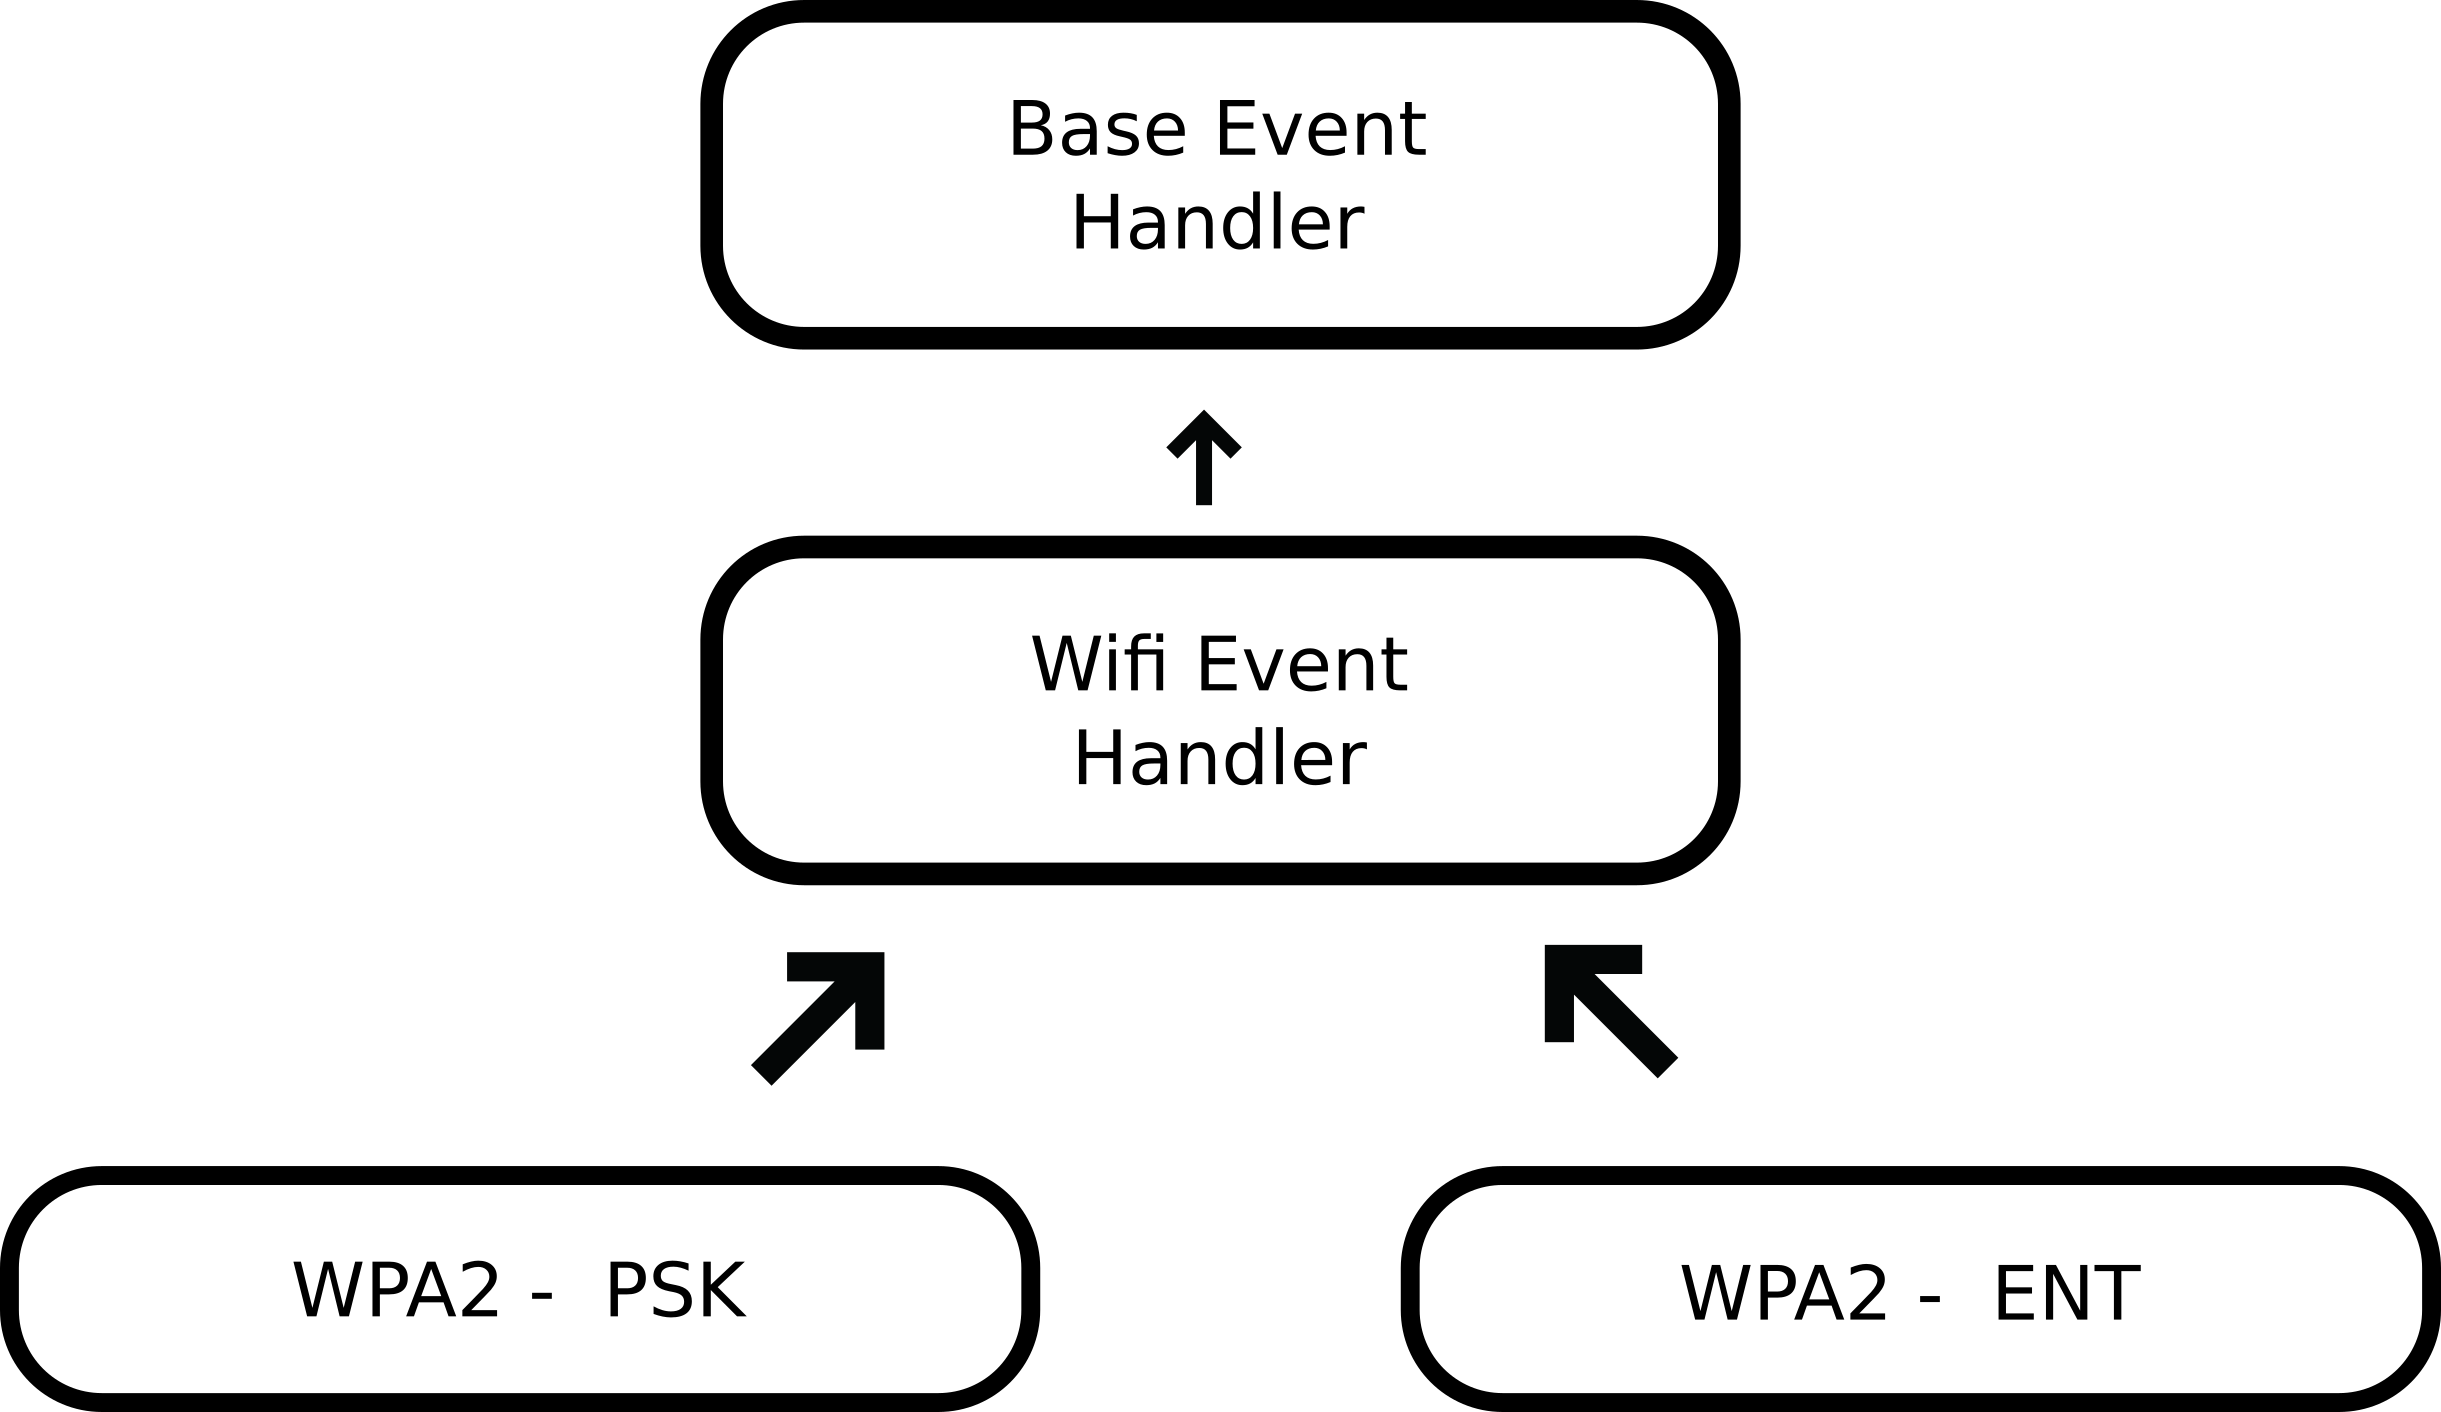
\includegraphics[scale=0.5]{figs/wifi-dia.png}
	\end{center}
	\caption{\label{fig:wifi} Diagrama de herança das classes da biblioteca wifi.} 
\end{figure}

\section{ESP-MQTT}

Responsável por controlar a comunicação \ac{MQTT} como um todo. A maneira utilizada para implementar o protocolo se 
baseia no sistema de eventos, onde cada evento está relacionado com uma etapa do estabelecimento da comunicação, 
porém as funções chamadas em cada um das etapas são métodos de uma classe que representa a conexão, de forma que 
a implementação da biblioteca em projetos futuros fique bem simples, se limitando a pouco mais do que instanciar o 
objeto e chamar o método \textit{PostData}. A \autoref{fig:mqtt} apresenta o modelo utilizado.

\begin{figure}[htb]
    \begin{center}
	    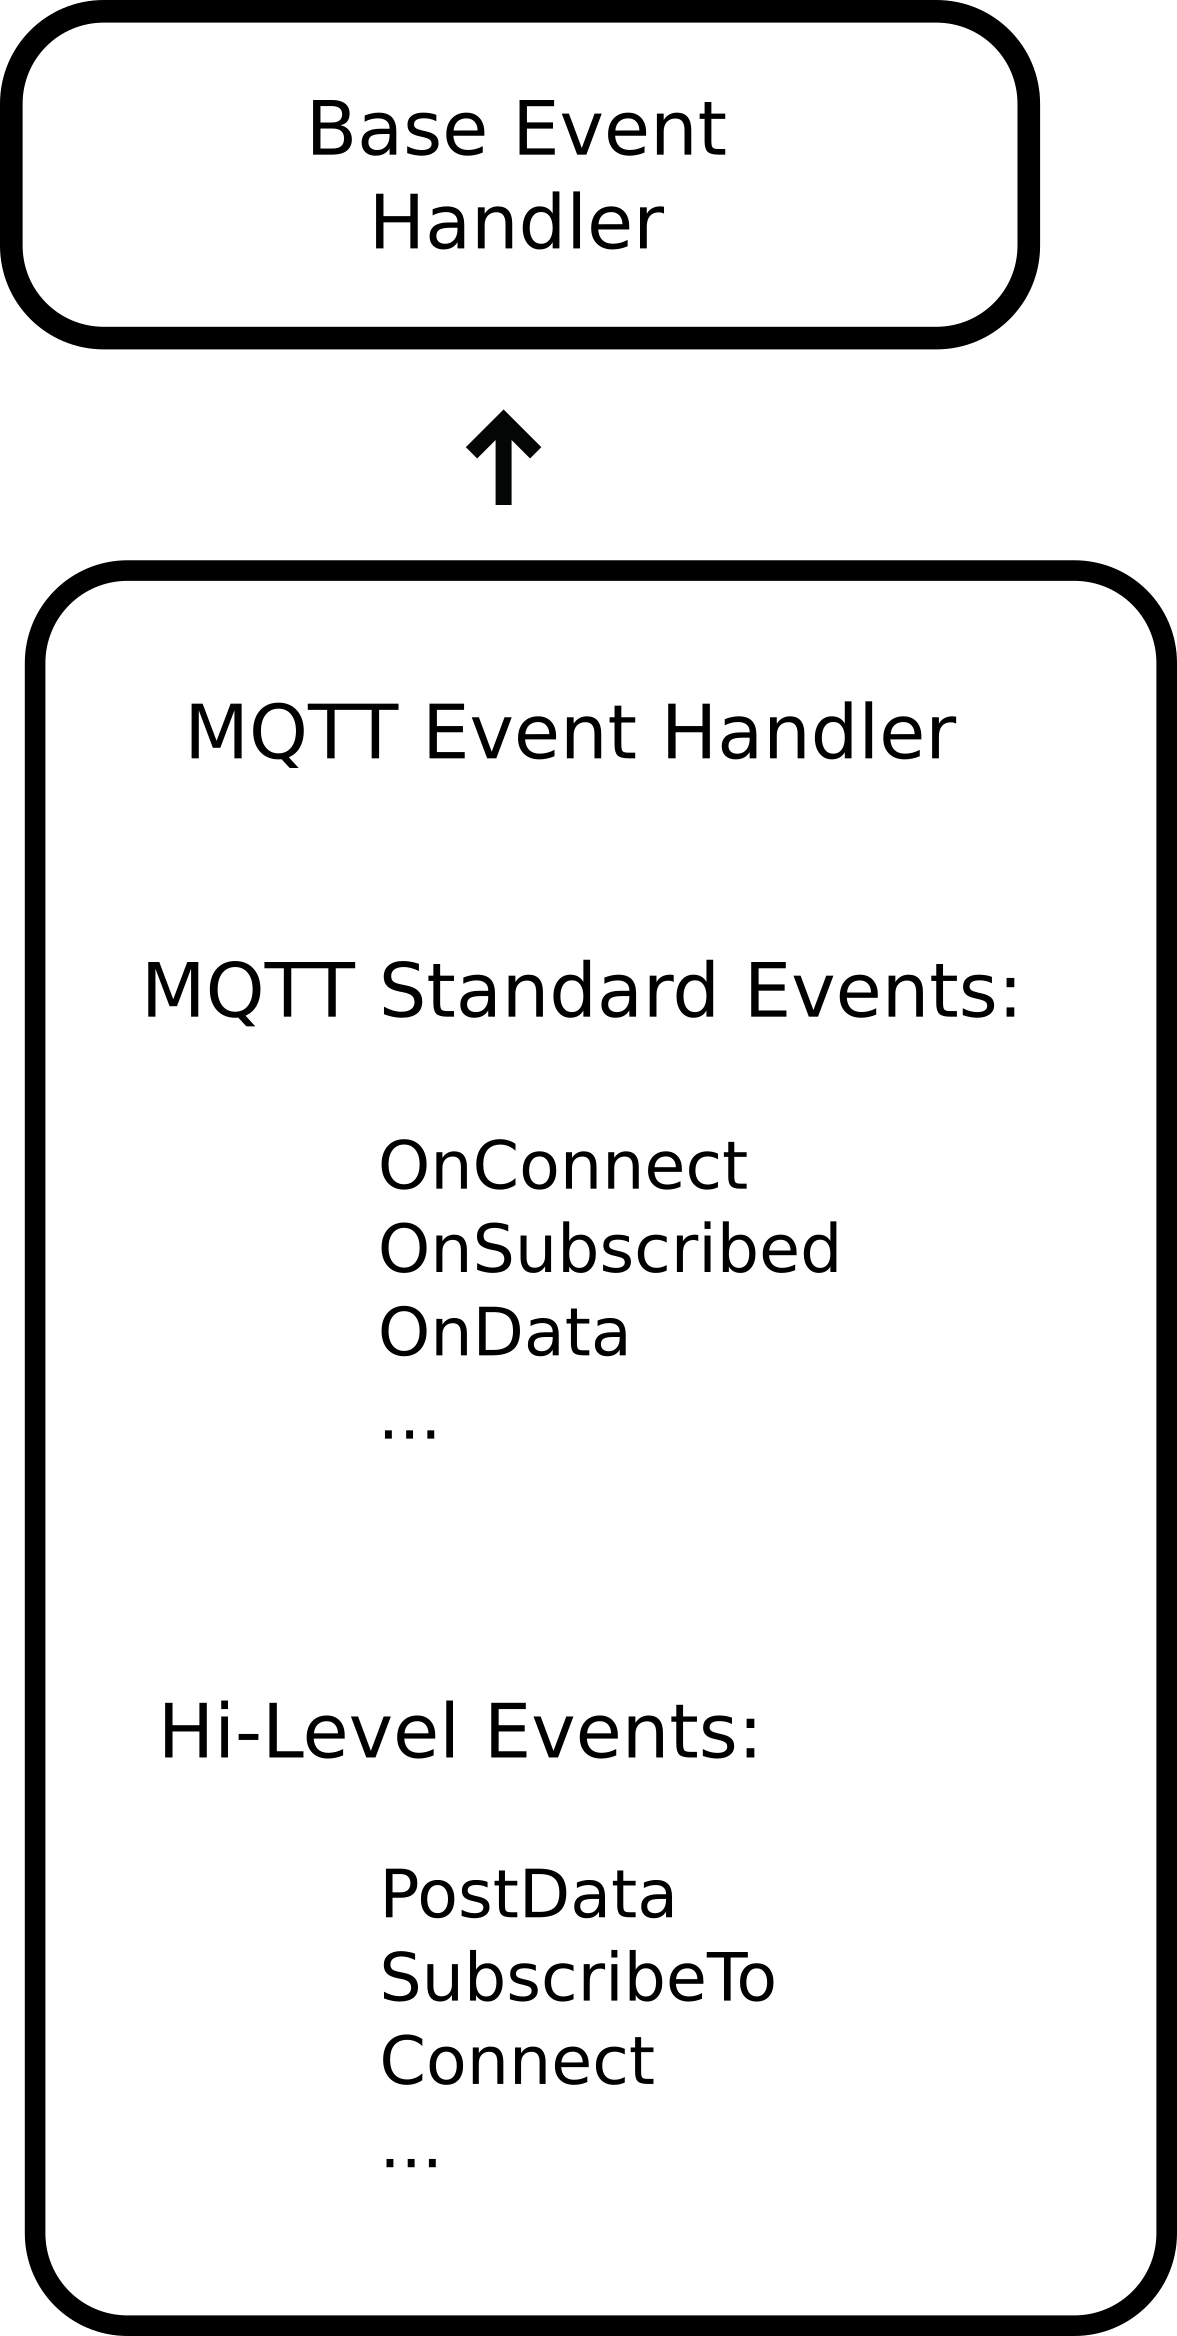
\includegraphics[scale=0.5]{figs/mqtt-dia.png}
	\end{center}
	\caption{\label{fig:mqtt} Diagrama esquemático da classe MQTT.} 
\end{figure}


\section{ESP-Serial}

Responsável por controlar a comunicação serial via \ac{UART} com diversos componentes. Do ponto de vista da arquitetura
ela segue os mesmos conceitos utilizados pela biblioteca responsável pelo \ac{MQTT} com as diferenças sendo basicamente
internas nas partes responsáveis pela instalação dos drivers para utilização dos pinos dos componentes.

\begin{figure}[htb]
    \begin{center}
	    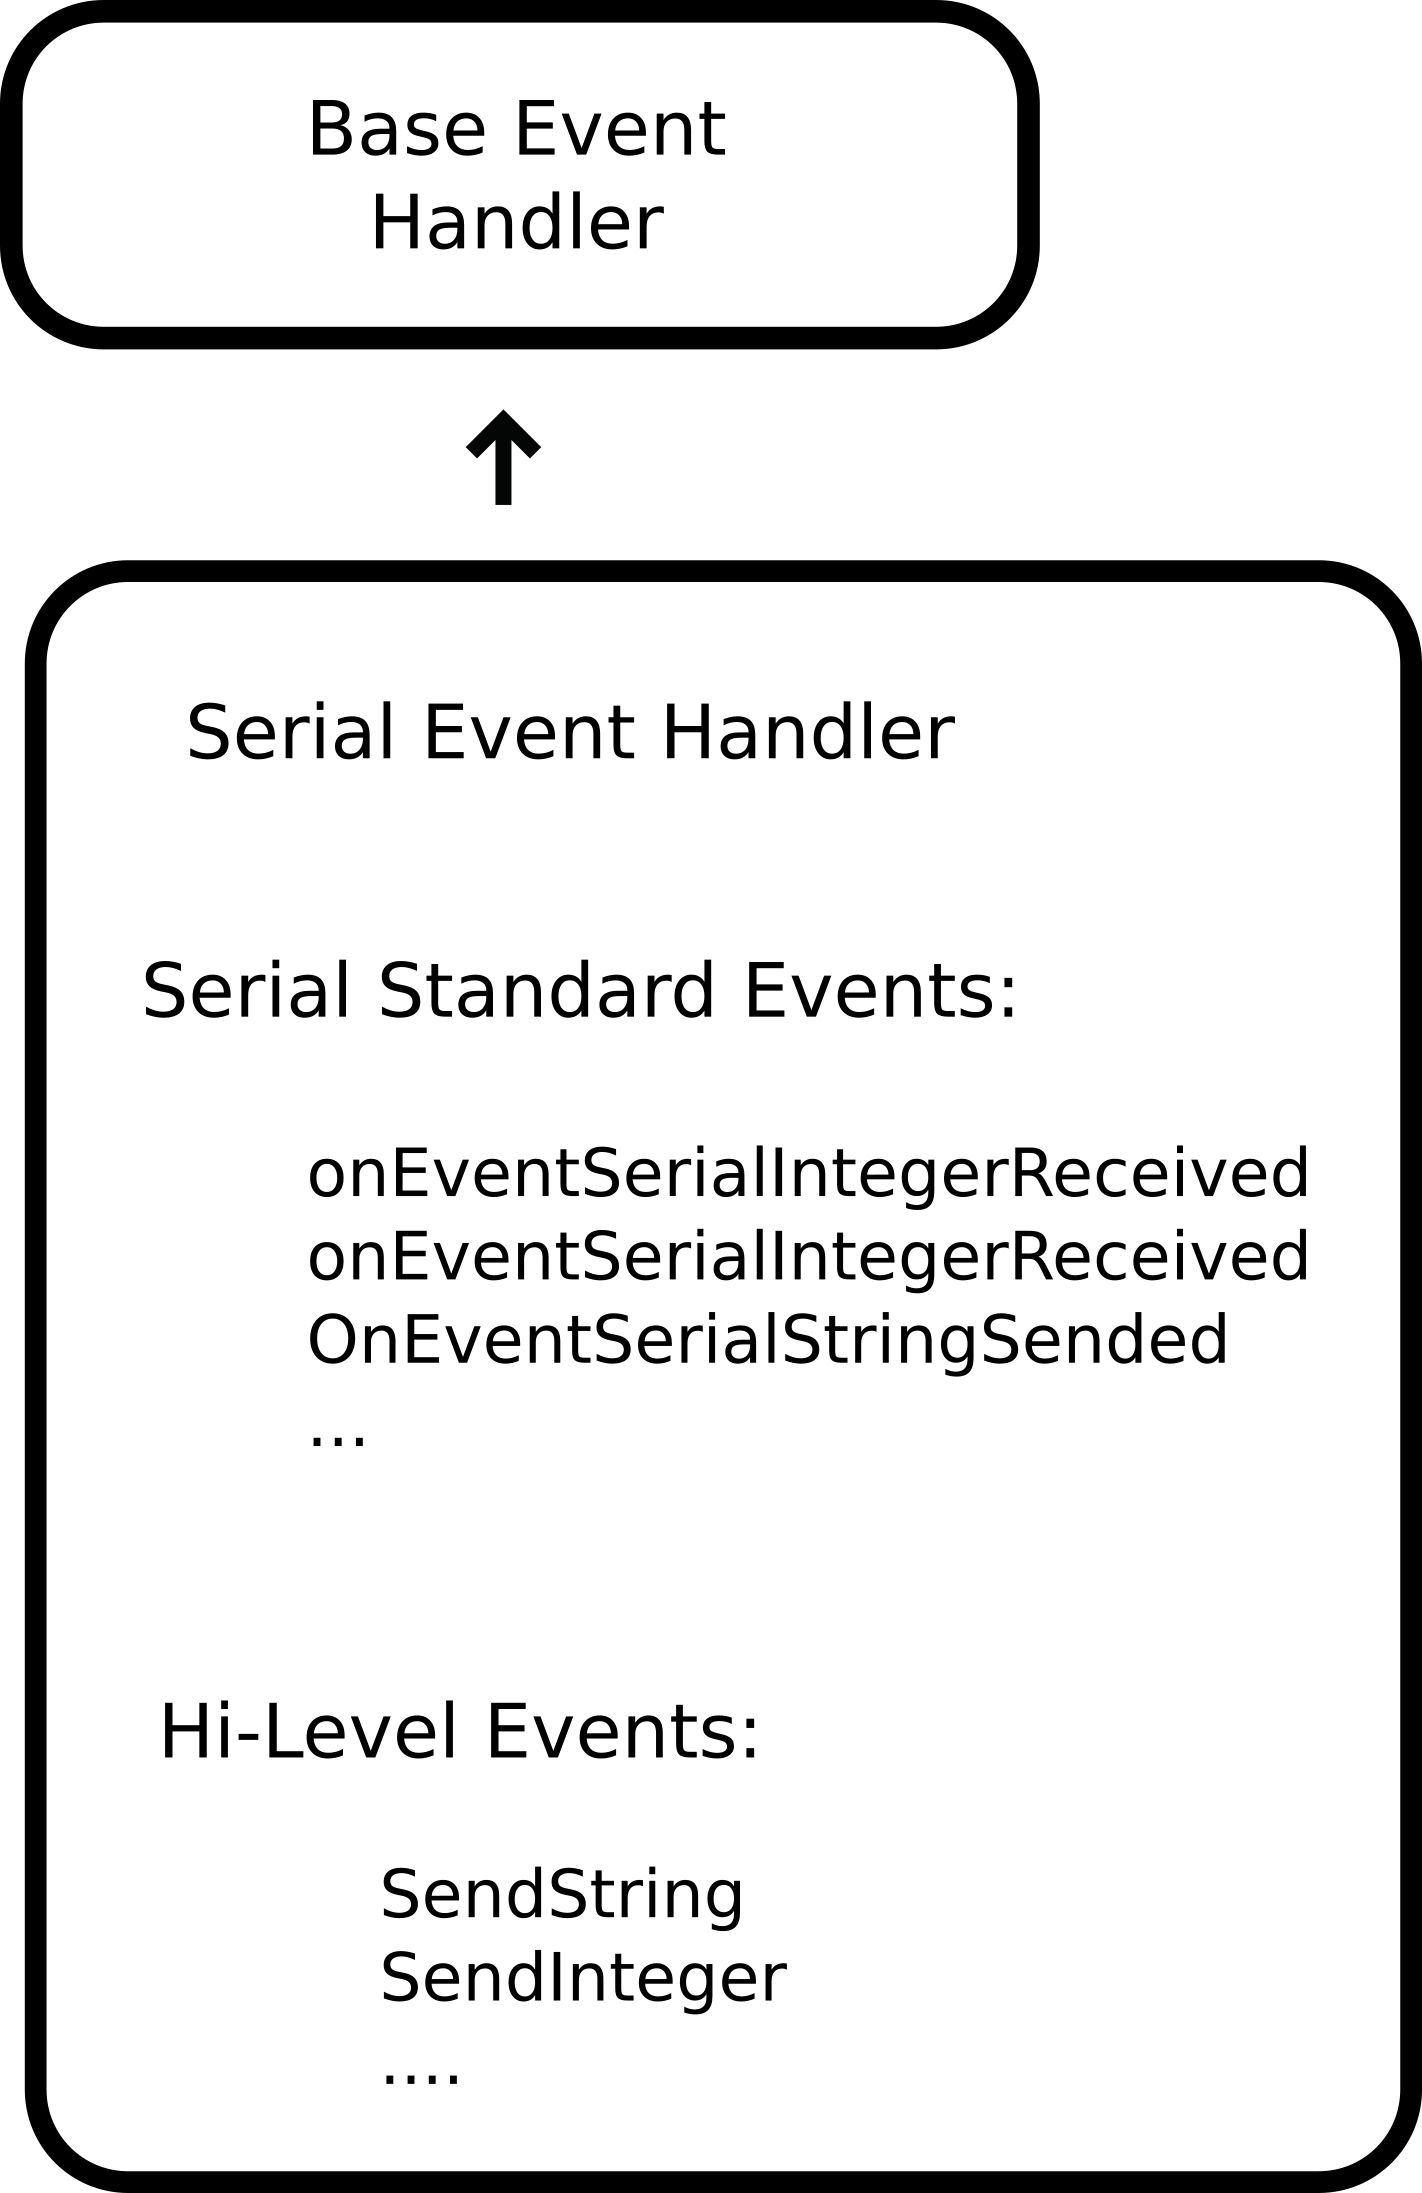
\includegraphics[scale=0.5]{figs/serial-dia.png}
	\end{center}
	\caption{\label{fig:serial} Diagrama esquemático da classe serial.} 
\end{figure}

\newpage
Uma colocação importante é a de que estas bibliotecas seguem o modelo de desenvolvimento dos componentes do \ac{ESP-IDF}
\footnote{O Framework de desenvolvimento dos ESP32 possui uma documentação bastante robusta e pode ser encontrada em 
\url{https://docs.espressif.com/projects/esp-idf/en/latest/esp32/index.html}\cite{esp-idf-docs}}
de forma que eles devem ser independentes e podem ser facilmente incorporados a códigos de terceiros
\footnote{Na documentação das bibliotecas no repositório existe um passo a passo de como essa importação pode feita 
utilizado somente um comando dos \textit{submodules} do GIT \cite{mapl-repo}}, mas que quando utilizados em conjunto 
apresentam ganhos, pois o fato de utilizarem a mesma classe mãe garante que eles utilizem somente um \textit{loop} de 
eventos e, portanto, menos recursos em memória já que na implemetação do \ac{ESP-IDF} todos os \textit{loops} de eventos
possuem no mínimo uma task em memória associada. 

Por fim, um segundo objetivo deste trabalho é propor um modelo de comunicação que possua meios para garantir a comunicação
local, diretamente via \ac{MQTT}, mesmo no caso de falhas dos servidores em nuvem, para isso incluir-se-á a descrição da 
configuração do \textit{Broker} mosquitto para tal.


